\iffalse
\documentclass[journal,12pt,twocolumn]{IEEEtran}
\usepackage{amsmath,amssymb,amsfonts,amsthm}
\usepackage{txfonts}
\usepackage{tkz-euclide}
\usepackage{listings}
\usepackage{gvv}
\usepackage[latin1]{inputenc}
\usepackage{array}
\usepackage{pgf}
\usepackage{lmodern}

\begin{document}
\bibliographystyle{IEEEtran}

\title{DISCRETE 11.9.3 Q-4}
\author{EE23BTECH11066 - Yakkala Amarnath Karthik
}
\maketitle

\bibliographystyle{IEEEtran}
\textbf{Question:} \\ \\The $4^{th}$ term of a G.P. is square of its second term, and the first term is -3. Determine its $7^{th}$ term.\\ \\
\textbf{Solution:}
\fi
\begin{table}[h!]
  \centering
    \begin{tabular}{|c|c|c|}
    \hline
    \textbf{Variable} & \textbf{Description} & \textbf{value}\\
    \hline
    $x(0)$ & first term of G.P. & -3 \\
    \hline
    $r$ & Common ratio of G.P. & ? \\
    \hline
    $x(n)$ & general term of the G.P. & $x\brak0r^{n}$ \\
    \hline
    $x\brak3$ & fourth term & $\sbrak{x\brak1}^2$\\
    \hline
    $u\brak{n}$ & unit step function & - \\
    \hline
  \end{tabular}

  \caption{A Table with input parameters}
  \label{tab:11.9.3.4.1}
\end{table}
from \tabref{tab:11.9.3.4.1}
\begin{align}
 x\brak0r^{3}&=\brak{x\brak0r^{1}}^2\\
 &=x\brak0^2r^2\\
\implies r&=x\brak0\\
&=-3
\end{align}
general term
\begin{align}
x\brak{n}&=x\brak0r^nu\brak{n}\\
&=\brak{-3}^{n+1}u\brak{n}
\end{align}
The $7^{th}$ term of the sequence will be:
\begin{align}
x\brak6 & =\brak{-3}\brak{-3}^{6}\\
& =-2187
\end{align}
Z transform of the given G.P is:
\begin{align}
X\brak{z}=\frac{x\brak0}{1-rz^{-1}}= \frac{-3}{1+3z^{-1}}.\hspace{0.5cm} |z|>3
\end{align}
\bigskip
\begin{figure}[ht]
        \centering
        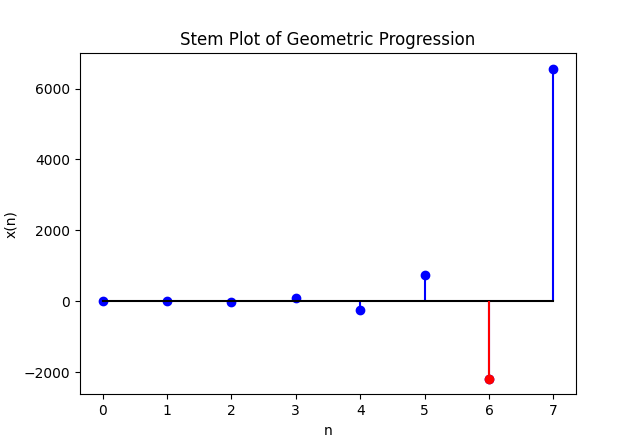
\includegraphics[width=0.45\textwidth]{ncert-maths/11/9/3/4/figs/stemplotfinal.jpeg}
        \caption{Graph showing first 8 terms of the GP}
    \end{figure} \\
%\end{document}
